%!TEX root = ../schoedon.tex

\cleardoublepage
\chapter{Overview and related work}
  \label{chap:overv}

  Table \ref{tab:overv:relat} (page \pageref{tab:overv:relat}) shows a first
  overview of related graphics, applications and publications in the broad
  field of mobility analytics and accessibility mapping techniques with focus
  on isochronic visualization techniques, reachability analysis and
  network-based approaches.\par

  \begin{table}[htp]
    \tiny \centering
    \begin{tabular}{r|l|l|l}
      \textbf{Year}
        & \textbf{Authors}
        & \textbf{Contribution}
        & \textbf{Type} \\
      \hline
      1881
        & Galton \cite{galton1881construction}
        & Construction of isochronic passage-charts
        & Publication \\
      1959
        & Hansen \cite{hansen1959accessibility}
        & How accessibility shapes land use
        & Publication \\
      1972
        & Armstrong \cite{armstrong1972network}
        & Network analysis of airport accessibility
        & Publication \\
      1978
        & Muller \cite{muller1978mapping}
        & Mapping of travel times
        & Publication \\
      1981
        & Sugiura \cite{Sugiura1981}
        & Japan travel time maps
        & Graphic \\
      1986
        & Hall \cite{hall1986fastest}
        & Network with random time-dependent travel times
        & Publication \\
      1989
        & Cauvin et al. \cite{cauvin1989cartographic}
        & The piezopleth maps method
        & Publication \\
      1993
        & Spierkermann et al. \cite{spiekermann1993zeitkarten}
        & Time maps for spatial planning
        & Publication \\
      1994
        & Spierkermann et al. \cite{spiekermann1994new}
        & Time-space maps of Europe
        & Publication \\
      1996
        & Gutierrez et al. \cite{gutierrez1996accessibility}
        & Accessibility analysis of the European road network
        & Publication \\
      1998
        & Fritz et al. \cite{fritz1998accessibility}
        & Accessibility as wilderness indicator
        & Publication \\
      1998
        & Juli{\~a}o \cite{juliao1998measuring}
        & Measuring accessibility with \acrshort{gis}
        & Publication \\
      1999
        & Miller \cite{miller1999measuring}
        & Measuring space-time accessibility within transportation networks
        & Publication \\
      1999
        & Spiekermann \cite{spiekermann1999visualisierung}
        & Visualization of railway travel times
        & Publication \\
      2000
        & Miller et al. \cite{miller2000gis}
        & \acrshort{gis} for measuring space-time accessibility in
          transportation
        & Publication \\
      2000
        & O'Sullivan et al. \cite{o2000using}
        & Using desktop \acrshort{gis} for accessibility analysis in public
          transport
        & Publication \\
      2001
        & Ran \cite{ran2001method}
        & Method of providing travel time
        & Patent \\
      2001
        & Handy \cite{handy2002accessibility}
        & Accessibility versus mobility
        & Publication \\
      2002
        & Lovett et al. \cite{lovett2002car}
        & Accessibility of general practitioner services
        & Publication \\
      2003
        & Altmaier et al. \cite{Altmaier2003}
        & Applications for inter-operable 3D geo-visualization
        & Publication \\
      2003
        & Dailey et al. \cite{dailey2003design}
        & Multi-modal transit management system
        & Publication \\
      2005
        & Auxhausen \cite{axhausen2005zeitkarten}
        & Time-maps of Switzerland
        & Publication \\
      2005
        & Chronomap \cite{Chronomap}
        & Drive-time analysis
        & Application \\
      2005
        & Karlin \cite{Karlin2005}
        & London subway travel times
        & Graphic \\
      2005
        & McLaren \cite{McLaren2005}
        & Time travel with the London tube map
        & Graphic \\
      2006
        & Lightfoot \cite{Lightfoot2006}
        & Use-cases for travel time maps
        & Publication \\
      2006
        & Pfoser et al. \cite{pfoser2006dynamic}
        & Dynamic travel time maps
        & Publication \\
      2006
        & Rüegg \cite{Ruegg2006}
        & Impact of public transport on travel times
        & Poster \\
      2006
        & Street \cite{street2006timecontours}
        & Isochrone visualization to describe transport network costs
        & Master's Thesis \\
      2006
        & Travel Time Tube Map \cite{Carden2006}
        & Interactive travel time tube map
        & Application \\
      2007
        & Brabec et al. \cite{Brabec2007}
        & Client-based spatial web-browsing
        & Publication \\
      2007
        & Irving \cite{Irving2007}
        & Use-cases for travel time maps
        & Publication \\
      2007
        & Nies et al. \cite{neis2007webbasierte}
        & Web-based accessibility analysis
        & Publication \\
      2008
        & Bauer et al. \cite{bauer2008computing}
        & Isochrones in multi-modal transportation networks
        & Publication \\
      2008
        & Mapumental \cite{Mapumental}
        & Maps that show time
        & Application \\
      2008
        & Uchida et al. \cite{Uchida2008}
        & Travel time to major cities
        & Graphic \\
      2009
        & FreeMapTools \cite{Freemaptools}
        & How far can I travel
        & Application \\
      2009
        & Uchida et al. \cite{uchida2009agglomeration}
        & Measure of urban concentration
        & Publication \\
      2010
        & Antrim et al. \cite{antrim2013many}
        & Use-cases for \acrshort{gtfs} data
        & Publication \\
      2010
        & Campenhout \cite{van2010travel}
        & Travel time maps
        & Master's Thesis \\
      2010
        & Glander et al. \cite{Glander2010}
        & Accessibility maps to visualize quality of mobility
        & Publication \\
      2010
        & Lei et al. \cite{lei2010mapping}
        & Mapping transit-based access
        & Publication \\
      2010
        & Marciuska et al. \cite{marciuska2010determining}
        & determining objects within isochrones
        & Publication \\
      2010
        & Müller et al. \cite{Mueller2010}
        & Distance transformations for accessibility mapping
        & Publication \\
      2010
        & Time Maps \cite{TimeMaps}
        & Public transport time maps of the Netherlands
        & Application \\
      2011
        & Birchler \cite{birchler2011computing}
        & Isochrones in multi-modal public transport networks
        & Bachelor's Thesis \\
      2011
        & Gemmel \cite{gemmel2012hedonic}
        & Effects of walk-ability and public transit
        & Master's Thesis \\
      2011
        & Gamper et al. \cite{gamper2011defining}
        & Defining isochrones in multi-modal spatial Networks
        & Publication \\
      2011
        & Isochrone.ch \cite{IsochroneCh}
        & Isochrones in schedule-based public transport
        & Application \\
      2011
        & Li et al. \cite{li2011dynamic}
        & Dynamic accessibility mapping
        & Publication \\
      2011
        & Söderström \cite{soderstrom2011personal}
        & Internet-driven maps based on time distances
        & Publication \\
      2011
        & Vaaraniemi et al. \cite{Vaaraniemi2011}
        & Rendering of high-quality cartographic roads
        & Publication \\
      2012
        & Byrd \cite{Byrd2012}
        & Visualizing urban accessibility
        & Publication \\
      2012
        & Gamper et al. \cite{gamper2012scalable}
        & Computation of isochrones with network expiration
        & Publication \\
      2012
        & Conveyal \cite{Conveyal}
        & Transportation - land use analysis
        & Application \\
      2012
        & Hollburg et al. \cite{hollburghier}
        & Interactive accessibility analysis in Potsdam
        & Publication \\
      2012
        & Mapnificent \cite{Mapnificent}
        & Web-based reachability visualization of public transport
        & Application \\
      2012
        & Mertens \cite{meertens2012}
        & Travel Time Maps of urban areas in the Netherlands
        & Graphic \\
      2012
        & Trevett \cite{Trevett2012}
        & 3D transmission format \acrshort{gltf}
        & Presentation \\
      2012
        & TripTropNYC \cite{TriptropNYC}
        & Web-based accessibility visualization in New York
        & Application \\
      2013
        & Efentakis et al. \cite{efentakis2013isochrones}
        & Reachability of population in urban catchment areas
        & Publication \\
      2013
        & Innerebner \cite{Innerebner2013}
        & Isochrones in multi-modal spatial networks
        & PhD Thesis \\
      2013
        & Innerebner et al. \cite{innerebner2013isoga}
        & Web-based geospatial reachability analysis tool
        & Publication \\
      2013
        & Transit Time NYC \cite{TransitTimeNYC}
        & Web-based subway transit times in New York
        & Application \\
      2013
        & Tran et al. \cite{tran2013go_sync}
        & Synchronizing transit data between \acrshort{gtfs} and \acrshort{osm}
        & Publication \\
      2014
        & Coughlin \cite{Coughlin2014}
        & 3D formats for the modern web
        & Publication \\
      2014
        & Gortana et al. \cite{gortanaisoscope}
        & Visualizing temporal mobility variance
        & Publication \\
      2014
        & Hollburg \cite{Hollburg2014}
        & Interactive analysis and visualization of accessibility
        & Master's Thesis \\
      2014
        & Isoscope \cite{Isoscope}
        & Visualizing mobility with isochrone maps
        & Application \\
      2014
        & Route360° \cite{Route360}
        & Web-based travel time analysis
        & Application \\
      2014
        & Krismer et al. \cite{krismer2014incremental}
        & Incremental calculation of isochrones
        & Publication \\
      2014
        & Voll \cite{vollerreichbarkeiten}
        & Accessibility analysis of the Alps
        & Publication \\
      2015
        & TravelTimePlatform \cite{TravelTimePlatform}
        & Search and filter by time not distance
        & Application \\
      2015
        & Trapp et al. \cite{Trapp2015}
        & Rendering transportation networks using distance fields
        & Publication \\
      2015
        & Yin et al. \cite{Yin2015}
        & Web-based accessibility analysis and travel time displays
        & Publication \\
      2016
        & Schoedon et al. \cite{STHD2016}
        & Web-based visualization of transportation networks
        & Publication \\
    \end{tabular}
    \caption{Selected related work.}
    \label{tab:overv:relat}
  \end{table}

  \section{Noteworthy publications and theses}
    \label{sec:overv:publc}

    \begin{figure}[ht]
      \subcaptionbox{
        \label{fig:overv:isopc}
        The Isochronic Passage Chart by Francis Galton, 1881
        \cite{galton1881construction}.}
      {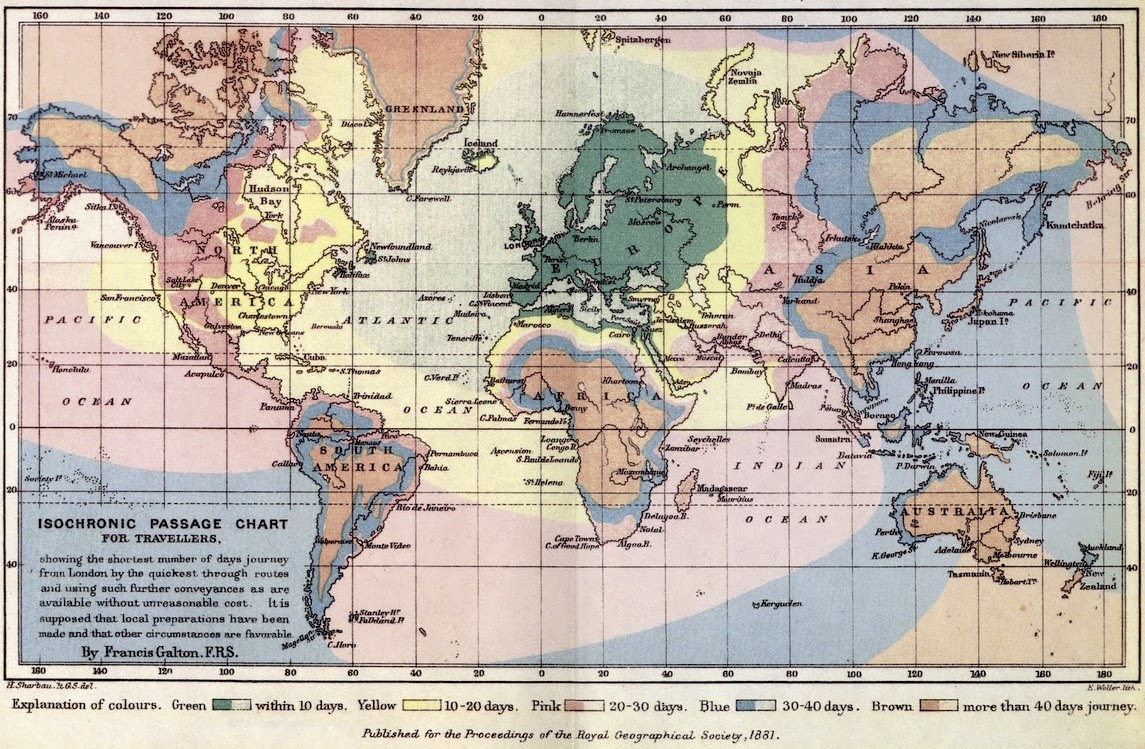
\includegraphics[width=0.32\textwidth]{./img/overv-isopc.jpg}}
      \hfill
      \subcaptionbox{
        \label{fig:overv:nodac}
        Analysis of Airport Accessibility in South Hampshire, 1972
        \cite{armstrong1972network}.}
      {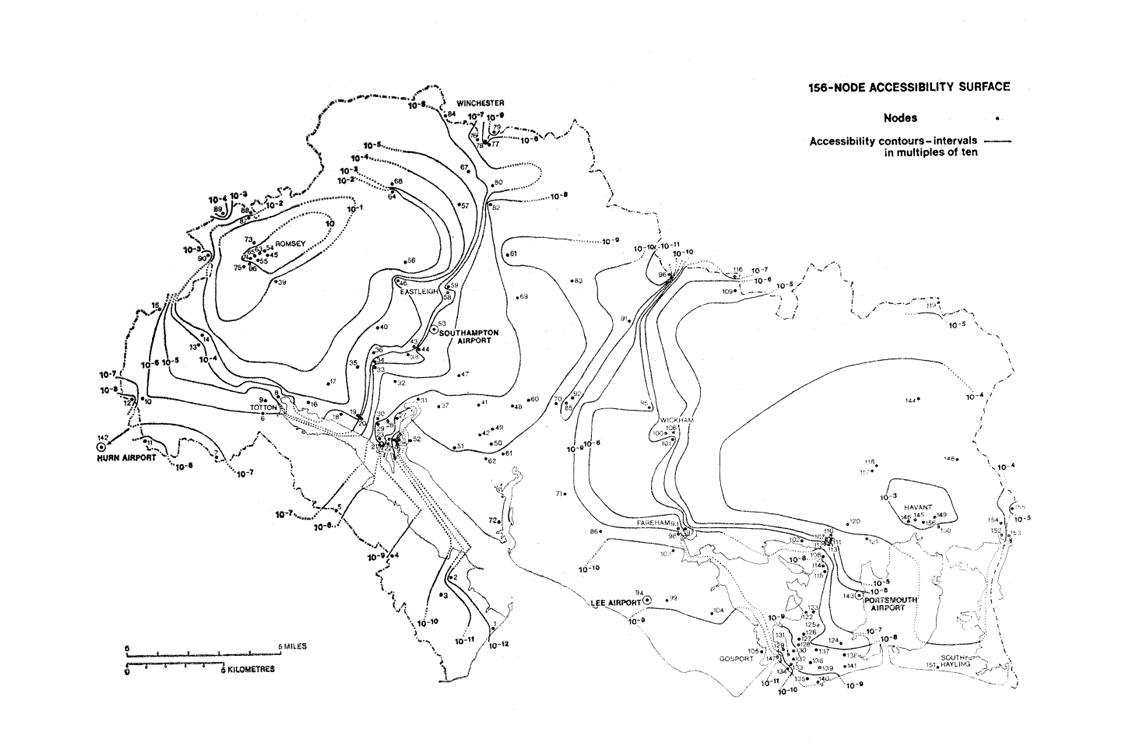
\includegraphics[width=0.32\textwidth]{./img/overv-nodac.png}}
      \hfill
      \subcaptionbox{
        \label{fig:overv:maptt}
        The Mapping of Travel Time in Edmonton, Alberta, 1978
        \cite{muller1978mapping}.}
      {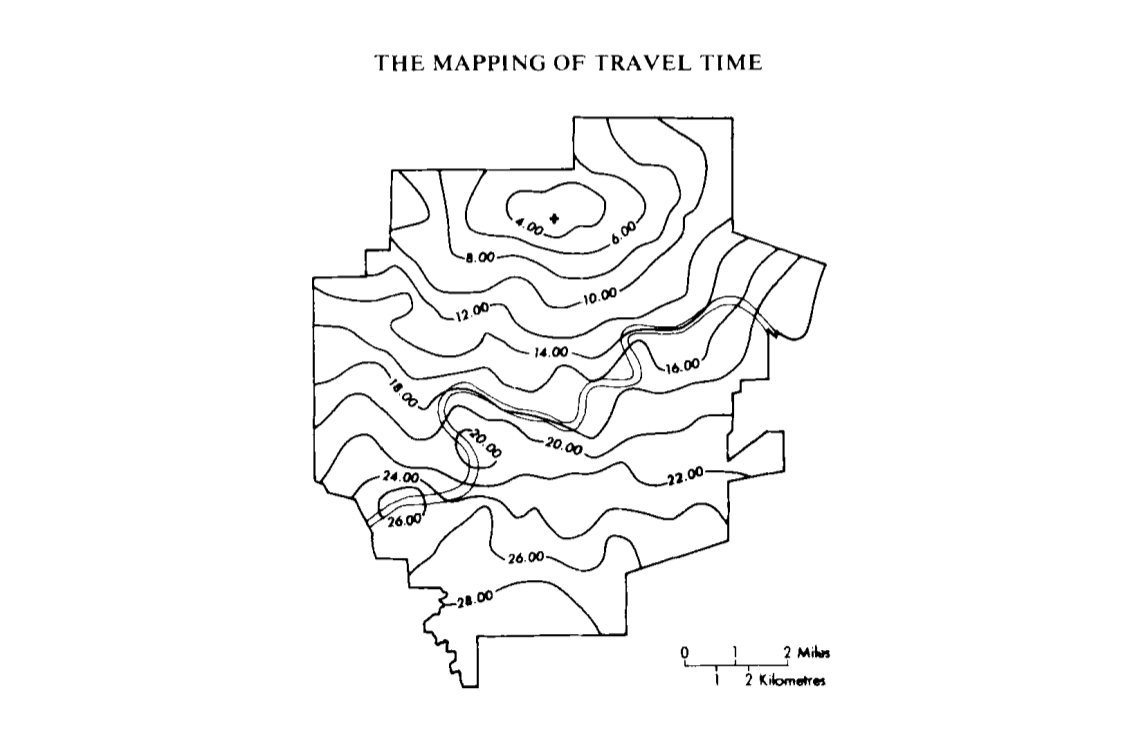
\includegraphics[width=0.32\textwidth]{./img/overv-maptt.png}}
      \label{fig:overv:1}
    \end{figure}

    In 1881, Francis Galton constructs the first isochronic map for the Royal
    Geographic Society (figure \ref{fig:overv:isopc}). It depicts the
    distances that can be traversed in equal times starting from London
    \cite{galton1881construction}. His contribution offers a polygonal
    generalization and suggests that future maps can be easily constructed for
    more detailed continental travel or home excursion maps.\par

    Among the first to define accessibility as indicator for urban
    transportation systems is Walter G. Hansen (1959). He presents a method for
    determining accessibility patterns within metropolitan areas and defines
    accessibility as the potential of opportunities for interaction serving
    residents in urban areas \cite{hansen1959accessibility}.\par

    % armstrong 1972
    % transport costs play an important role
    % here: economic evaluation of airports
    % road travel times and weighting by importance for the application
      % and population
    %%% GRAPHIC FIG 3or4

    Pioneer in computing accessibility analysis on the foundation of
    transportation networks is Harvey W. Armstrong (1972) who converts an
    exemplary road network with 159 nodes to a matrix and used a C.D.C. 6000
    computer to evaluate economic feasibility of airports in South Hamphsire
    \cite{armstrong1972network} (figure \ref{fig:overv:nodac}).\par

    Jean-Claude Muller (1978) highlights issues with the mapping of
    time-distances as the derived space is often non-euclidean and hardly
    mappable without distorting the geographic reference system
    \cite{muller1978mapping}. He presents a numerical approach for time-distance
    transformations of Edmonton and analyses the resulting distortions (figure
    \ref{fig:overv:maptt}).\par

    \begin{figure}[ht]
      \subcaptionbox{
        \label{fig:overv:patnt}
        Patent: Method of Providing Travel Time, 2001
        \cite{ran2001method}.}
      {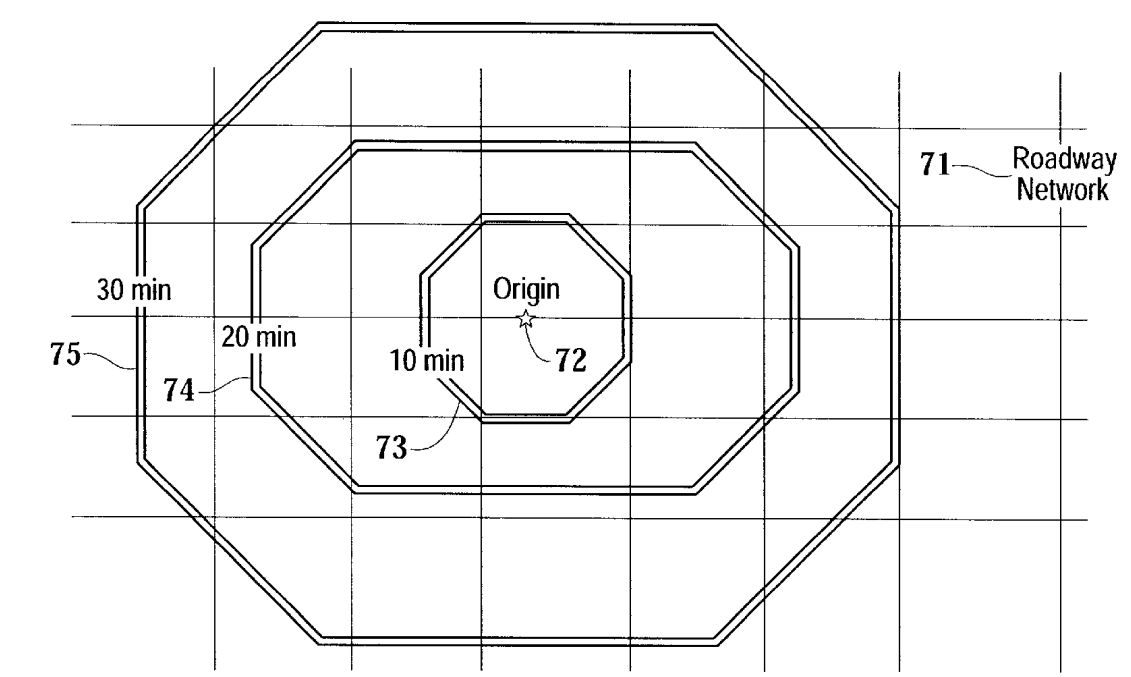
\includegraphics[width=0.32\textwidth]{./img/overv-patnt.png}}
      \hfill
      \subcaptionbox{
        \label{fig:overv:berln}
        Visualization of Quality of Mobility in Public Transport, 2010
        \cite{Glander2010}.}
      {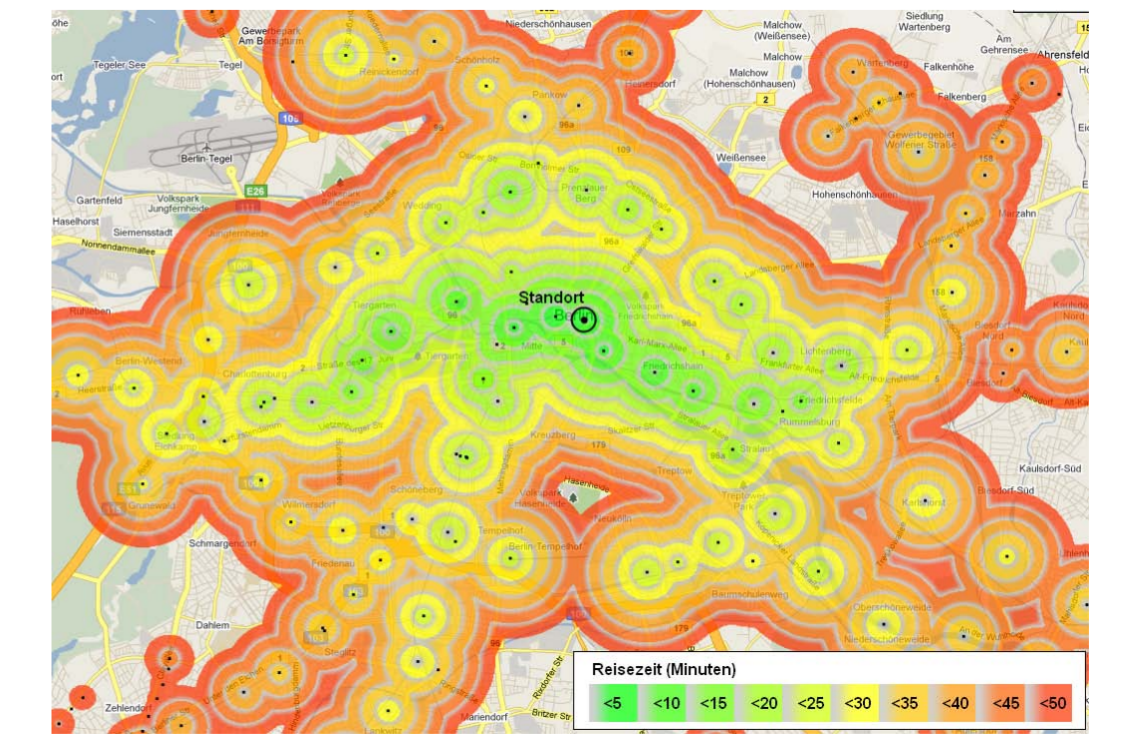
\includegraphics[width=0.32\textwidth]{./img/overv-berln.png}}
      \hfill
      \subcaptionbox{
        \label{fig:overv:potsd}
        Network-Based Accessibility Visualization in Potsdam, 2012
        \cite{hollburghier,Hollburg2014}.}
      {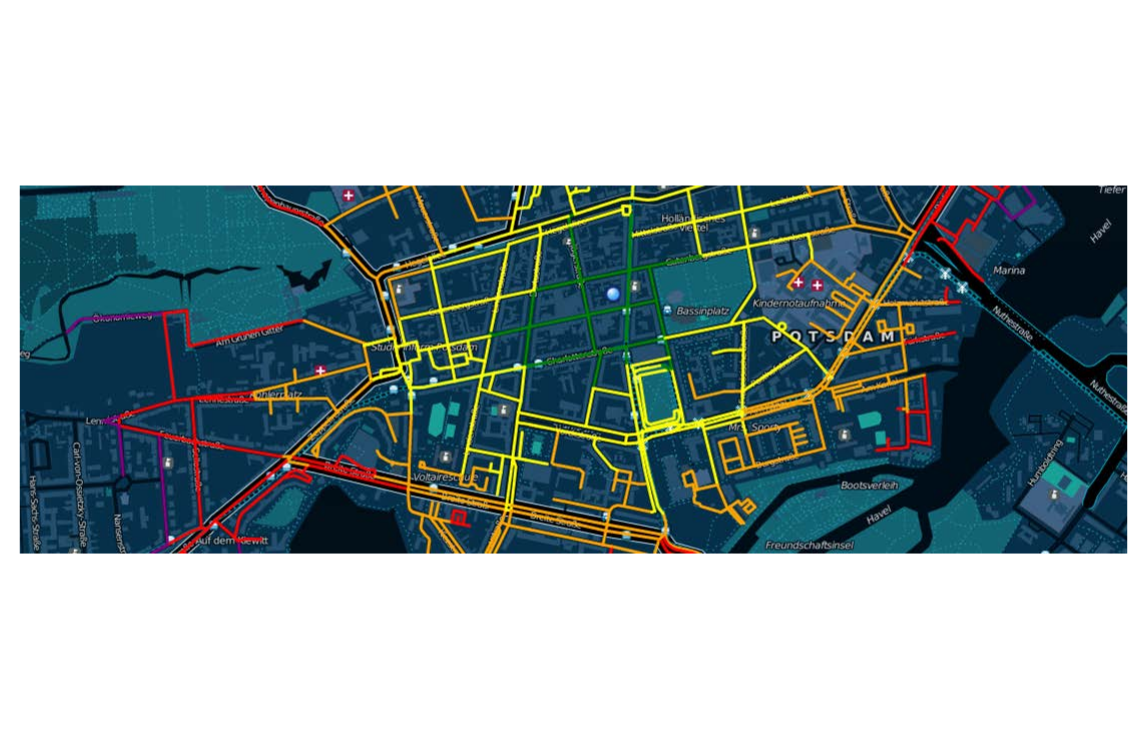
\includegraphics[width=0.32\textwidth]{./img/overv-potsd.png}}
      \caption{Shoo bar.}
      \label{fig:overv:2}
    \end{figure}

    The United States Patent and Trademark Office (\acrshort{uspto}) publishes
    the patent \#US006317686B1 issued by Bin Ran in 2001 on the method of
    providing travel time \cite{ran2001method}. It claims a personalized
    multi-modal travel prediction and trip decision support system including
    traffic forecast maps such as travel speed maps, travel time maps, and
    travel cost maps. It uses contour lines to represent predictive minimal
    travel time from a selected origin (figure \ref{fig:overv:patnt}).\par

    % street theis 2006
    % time based maps describe time accessibility of networks
    %%% FIG: 56 or 57 global integration of london (axial map) of network

    An important milestone and often cited reference is the final report on
    TimeContours by Nicholas Street (2006). It provides a Java application which
    maps isochrones onto public transport and road graphs to display
    transportation costs with respect to the travel time required
    \cite{street2006timecontours}. It discusses methods to display more than two
    dimensions on geographic maps such as isolines and defines isochrones --
    isolines of same time -- as derivation of the in topographic maps more
    commonly used isohypses -- isolines of the same height -- in a similar
    manner.\par

    % neis et al. 2007
    % utilizes attributed street network graph
    %%% FIG 13 accessibility maps buffer isolines convexhull

    A first web-based service for accessibility analysis is specified by
    Neis et al. (2007). Their approach suggests an accessibility analysis
    service (\acrshort{aas}) based on standards defined by the Open Geospatial
    Consortium (\acrshort{ogc}) \cite{neis2007webbasierte}. A provided web
    application is presented as Java Applet and receives responses in extensible
    markup language format (\acrshort{xml}). It calculates an elevation model
    where the third dimension encodes the required travel time and compares
    different visualization methods such as buffers, convex hulls and isochrones
    to display the results.\par

    A well organized summary on different methods for providing accessibility
    maps such as accessibility indices, anamorphosis maps or isochrone
    visualizations can be found in Martijn van Campenhout's thesis on travel
    time maps (2010) \cite{van2010travel}.\par

    % glander 2010
    % calculates isochrones from weighted voronoi centers (?)
      % and distance fields
    %%% FIG 1 public transport berlin

    % müller 2010
    % distance transformations for accessibility mapping
      % in public transport domain
    % for concurrent web based accessibility mapping
    % surface based (euclidean) vs network based (non euclidean)
      % distance computation
    % first who highlights: display of network is no only effective
      % for the user but efficient and correct calc'able
    % generalized polygons introduce visual errors and high rendering demand

    Glander et al. (2010) present an accessibility map visualization technique
    with a focus on polygon-based approaches in the public transport domain
    \cite{Glander2010} (figure \ref{fig:overv:berln}), and raster-based distance
    transforms~\cite{Mueller2010} which both lack precision in display offered
    by network-based approaches such as the one presented in this thesis
    (C\ref{enu:contr:c1}).\par

    % gortana 2014
    % FIG 1 24 layered shapes for each hour of the day

    % yin et al. 2015
    % integrated platform for accessibility analysis tasks
    % accessible to a wider range of audiences
    % FIG 4accessibility view (choropleth), travel time view (isochrone)

    The team around Yin et al. (2015) presents a web-based system for
    visualization of multi-modal accessibility for multiple land-uses. It
    highlights the importance of providing an easy-to-use web-interface as the
    users will not need to purchase or install software and therefore make the
    application accessible to a wider range of audiences~\cite{Yin2015}.
    However, the visualization technique does not focus on the specifics of
    transportation network representations.\par

  \section{Direct predecessors of this thesis}
    \label{sec:overv:predc}

    This thesis is furthering the work of Hollburg et al. (2012,
    2014) and the resulting services Motion Intelligence GmbH offers with their
    Route360°-\acrshort{js} \acrshort{api}. In \cite{hollburghier}, a web-based
    accessibility mapping service is provided to support tourists in assessing
    reachability for points of interest (\acrshort{poi}) in the city of Potsdam.
    It provides a
    limited network-based visualization and highlights the benefits from
    mapping the travel times directly onto the transportation network rather
    than calculating isochrones (figure \ref{fig:overv:potsd} on page
    \pageref{fig:overv:potsd}). However, it
    realizes it's not feasible to use this approach for larger networks
    including car travel or public transport (D\ref{enu:drawb:d3}).\par

    In \cite{Hollburg2014}, Hollburg
    presents an efficient way to generalize road segments (D\ref{enu:drawb:d1})
    and to calculate
    isochrones to visualize large accessibility maps in web clients and argues
    polygons are faster to transmit than complete network geometries due to the
    smaller data volume. The network-based method developed in his preceding
    work was comprehensible but not efficient for huge transportation networks.

  \section{Related applications and map graphics}
    \label{sec:overv:applc}

    % maps %%%%%%%%%%%%%%%%%%%%%%%%%%%%%%%%%%%%%%%%%%%%%%%%%%%%%%%%%%%%%%%%%%%%%

    % apps %%%%%%%%%%%%%%%%%%%%%%%%%%%%%%%%%%%%%%%%%%%%%%%%%%%%%%%%%%%%%%%%%%%%%

    Apart from the scientific work presented in sections \ref{sec:overv:publc}
    and \ref{sec:overv:predc}, a comprehensive overview of web applications
    and map graphics or map related representations is given in this
    section.\par

% 2006 Travel Time Tube Map \cite{Carden2006} & Interactive travel time tube map & Application
% among the first, web java applet, distorts london tube network by selected starting location
% maps static circle isocrhones, distortion to eucledian distances

% 2008 Mapumental \cite{Mapumental} & Maps that show time & Application
% isochrone for reachable area by public transport
% shadows area which is unreachable
% see also work by \cite{Lightfoot2006} \cite{Irving2007}

% 2009 FreeMapTools \cite{Freemaptools} & How far can I travel & Application
% Instead of a radius as the crow flies, can you do a radius as the car drives"
% calculates an isochrone "radius" based on speed and travel time on an actual road map

% 2010 Time Maps \cite{TimeMaps} & Public transport time maps of the Netherlands & Application
% similar to tom cardens tube map, it distorts a map of the netherlands
% based on public transport (railways), unique: displays different times of the day
% static circular isochrones, distorted basemap
% see also work by \cite{meertens2012}

% 2011 Isochrone.ch \cite{IsochroneCh} & Isochrones in schedule-based public transport & Application
% dedicated web application to display public transport accessibility in switzerland by isochrones
% see also work by birchler \cite{birchler2011computing}

% 2012 Conveyal \cite{Conveyal} & Transportation - land use analysis & Application
% logistics and land use with isochrones on quarter level
% multimodal, commercial web application

% 2012 Mapnificent \cite{Mapnificent} & Web-based reachability visualization of public transport & Application
% web application with simplified client-based routing & gtfs
% calculates isocrhone on the fly, shades unreachable areas
% multi-modal

% 2012 TripTropNYC \cite{TriptropNYC} & Web-based accessibility visualization in New York & Application
% calculates isochrones server-side and transmit them to teh client (warns user about the huge traffic impact)
% interesting method: buffers look like squares / rectangles
% public transport only

% 2013 Transit Time NYC \cite{TransitTimeNYC} & Web-based subway transit times in New York & Application
% approximates isochrones by displaying a grid of hexagons colored by average travel time
% public transport only

% 2014 Isoscope \cite{Isoscope} & Visualizing mobility with isochrone maps & Application
% isoscope web app at FH;P
% unified isochrone maps with time varying  travel data
% instead multiple isolines for for travel times: mult isolines for times of day
% reveals time-dependent spatial travel variance
% see also \cite{gortanaisoscope}

% 2014 Route360° \cite{Route360} & Web-based travel time analysis & Application
% polygonal travel time services, javascript api
% multi-modal, isochrones

% 2015 TravelTimePlatform \cite{TravelTimePlatform} & Search and filter by time not distance & Application
% time is the new distance, discover poi by reachable time, decide, route
% isochrones, multimodal
% FIG slider_sX

% walk score travel time api / drive time api
% multimodal traveltimes, including/excluding traffic
% dynamic visualizations, fixed polygons (isocrhones)
% https://www.walkscore.com/professional/travel-time-api.php

% trulia maps commute time, 60min max, public transport + car (isochrones)
% http://www.trulia.com/local/los-angeles-ca/driving:1|transit:0|position:34.052218;-118.243389|time:60_commute

% simplefleet
% isochrones, statistics on reachable population
% http://www.simplefleet.eu/?page_id=54

% public transit travel time geoss.colorado.edu/traveltime/
% geoss.colorado.edu/traveltime/TravelTime.pdf
% http://i.imgur.com/QrWOfJ3.png
% https://www.fastcoexist.com/3025581/visualized/these-maps-redraw-cities-based-on-how-long-it-takes-to-get-around-without-a-car
% anymations https://www.youtube.com/watch?v=CMazGQHsMEM&feature=youtu.be&t=27s.

% Open route service accessibility analysis
% isochrone methods: recursive grid, TIN
% slowwwww, ugly, buggy
% http://www.openrouteservice.org/

% OneBayArea Maps, San Fransisco Plan 2040
% isochronen auf viertel-ebene (blocks), single use case
% http://maps.planbayarea.org/travel_housing/

% Graphhopper Direction API
% Isochrone API, simple isochrones
% https://graphhopper.com/api/1/docs/isochrone/

% Mapbox OSRG Isochrone plugin
% https://github.com/mapbox/osrm-isochrone

% Isochronous Application
% simple single isochrone, queried from google maps server, buggy
% http://cartoo.dyndns.org/




% https://www.khronos.org/news/press/significant-gltf-momentum-for-efficient-transmission-of-3d-scenes-models

